\documentclass[Arkitektur/System_main.tex]{subfiles}
\begin{document}
\subsection{Security View}
I dette afsnit beskrives de aspekter der er i forhold til sikkerhed i systemet. Der beskrives hvordan sensibel data håndteres, hvad der gør for brugersikkerhed og hvordan der autoriseres så kun brugere med rette autorisering kan tilgå dele af systemet. Afsnittet fokuserer på systemet ud fra en vinkel med fokus på sikkerhed og hvordan sikkerhed påvirker systemet.
\subsubsection{Koncepter om brugersikkerhed}
Da denne applikation håndterer sensibel data om sine brugere i form af navne, adresser, registreringsnummer på biler osv., så er det vigtigt at opretholde en form for sikkerhed omkring brugernes konti. Den nemmeste måde at få adgang til disse oplysninger er gennem brugerkontiens adgangskode og derfor tages der nogle foranstaltninger omkring denne. \begin{itemize}
    \item Brugerens adgangskode holdes ikke i hukommelsen af programmet. 
    \item Brugeren påduttes en adgangskodesikkerhed ved, at adgangskoden skal indeholde både tal og bogstaver.
    \item Brugeren påduttes en adgangskodesikkerhed ved, at adgangskoden skal være længere end 6 karakterer.
    \item Brugerens adgangskode opbevares ikke i ren tekst på en database.
\end{itemize}

Når en bruger skal ændrer, tilføje eller slette information går det over en sikker https-forbindelse, der sender krypteret data til applikationsserveren. Det samme gør sig gældende, når en bruger skal sende information til en anden bruger. Dette afspejles i figur \ref{fig:security_diagram_first}.
\begin{figure}[H]
    \centering
    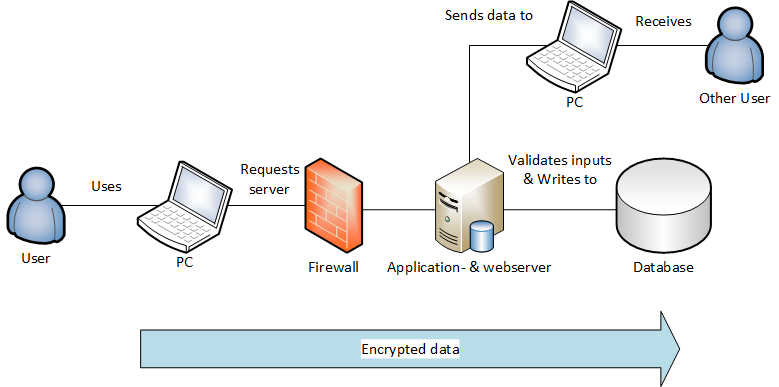
\includegraphics[width=\textwidth]{Arkitektur/graphics/SecurityDiagramFirst.png}
    \caption{Securitydiagram for simpel bruger-til-bruger og bruger-til-server interaktion}
    \label{fig:security_diagram_first}
\end{figure}
Denne type arkitektur anvendes i de tidlige stadier, da den er simplest at udvikle på, men den er dårlig i et produktionsmiljø, da hvis en ting fejler, så fejler hele systemet. Derfor specificeres en N-tier arkitektur\footnote{https://www.synopsys.com/blogs/software-security/attributes-of-secure-web-application-architecture/}, der efter udviklingen af den først arkitektur, kan arbejdes henimod. Denne ses på figur \ref{fig:security_diagram}.

\begin{figure}[H]
    \centering
    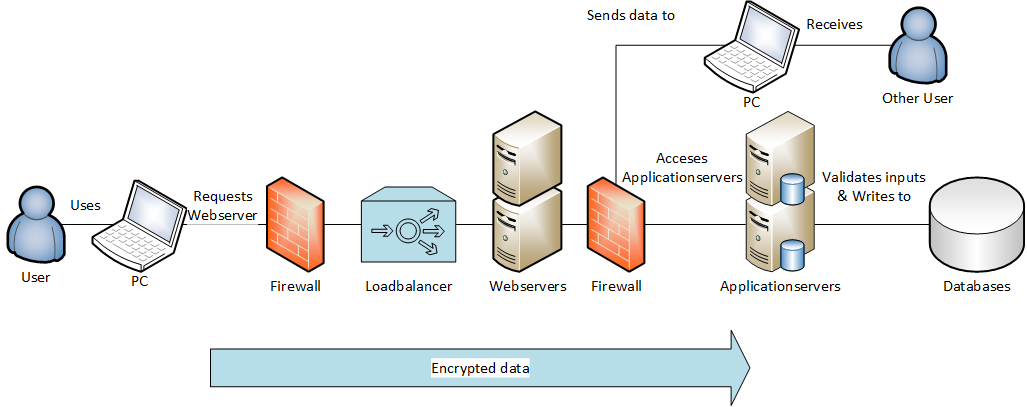
\includegraphics[width=\textwidth]{Arkitektur/graphics/SecurityDiagram.png}
    \caption{Securitydiagram for produktions bruger-til-bruger og bruger-til-server interaktion}
    \label{fig:security_diagram}
\end{figure}

Grunden til at denne måde er at fortrække i et produktionsmiljø er at en eventuel trussel ikke kan nedlægge hele systemet ved at nedlægge en enkelt webserver.

\subsubsection{Koncepter om validering}
Når man har brugerinputs i sin applikation skal disse valideres for at forhindre eventuelle trusler i form af ondsindede brugerinputs. Dette kan ske hos klienten (altså i applikationen), på serveren eller på begge. Validering hos klienten aflaster serveren og giver derved bedre serverperformance. Derfor valideres email om det er en valid email og password om det opfylder kravene på applikationen (clientside). Når dette er gjort sendes bruger inputs til serveren, hvor de valideres inden videre behandling. Valideringerne kan ses visualiseret i figur \ref{fig:datavalidation_diagram}.

\begin{figure}[H]
    \centering
    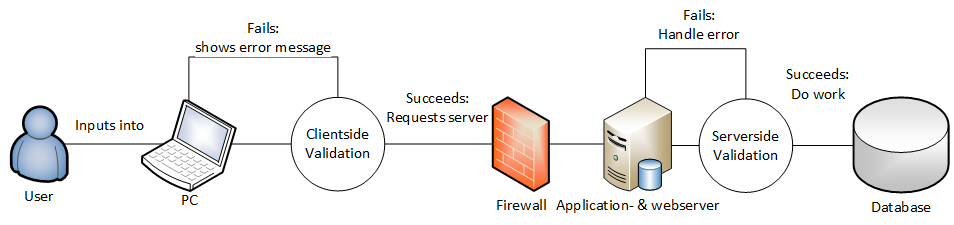
\includegraphics[width=\textwidth]{Arkitektur/graphics/DataValidationDiagram.png}
    \caption{Datavalidationdiagram for clientside og serverside valideringer}
    \label{fig:datavalidation_diagram}
\end{figure}


\end{document}